\documentclass[tikz,border=0]{standalone} 
\usepackage{tikz}
\usetikzlibrary{trees}
\usetikzlibrary{shadows}
\begin{document}
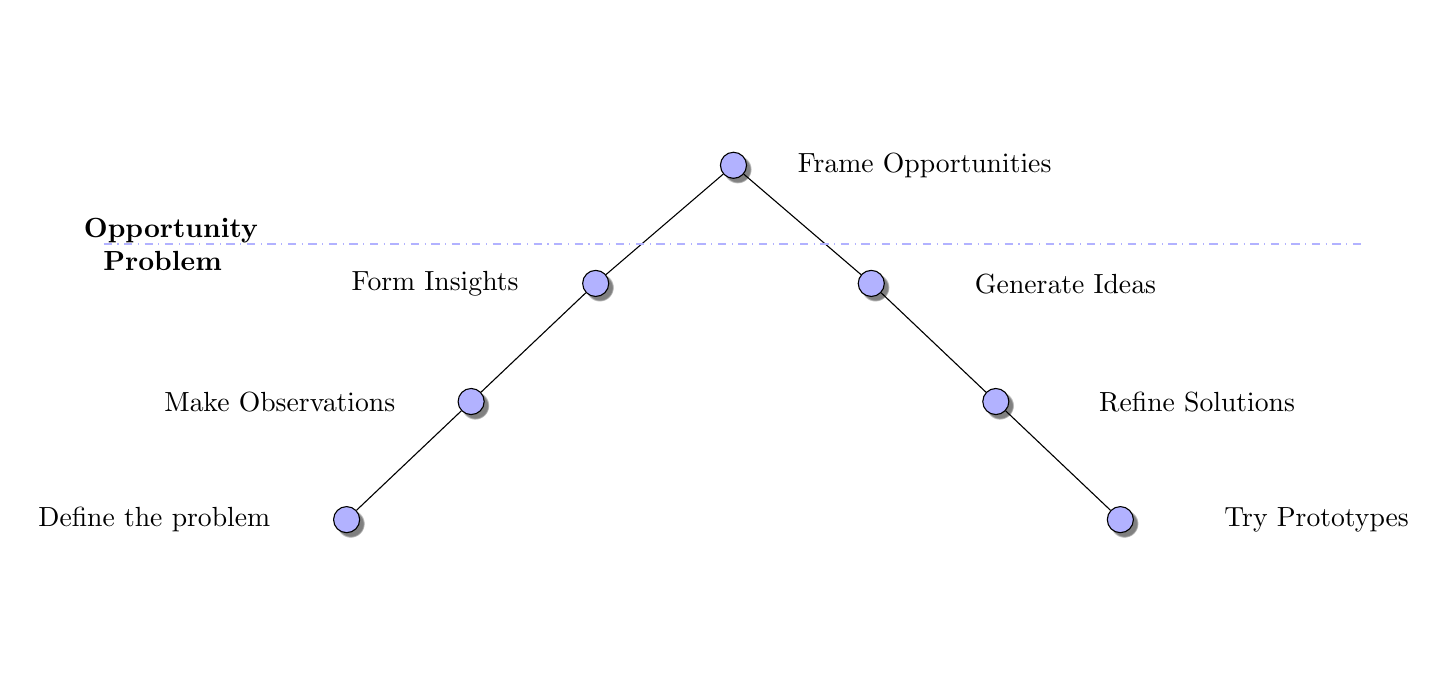
\begin{tikzpicture}[level distance=1.5cm,
level 1/.style={sibling distance=3.5cm},
level 2/.style={sibling distance=1cm}]
\tikzstyle{every node}=[circle, draw, fill=blue!30]
% Preamble:
\tikzset{no shadows/.style={general shadow/.style=}}
every label/.append style = {
     label distance=1em,
     font=\scriptsize,
     every shadow/.style={opacity=0}, % <- add this
  }
\node (Root) [circular drop shadow, label={[label distance=0.5cm]0:Frame Opportunities}] {}
    child {
    node[circular drop shadow, label={[left, label distance=-1cm]0:Form Insights}] {} 
    child { 
        node[circular drop shadow, xshift=-4.5em, label={[left, label distance=-1cm]0:Make Observations}] {} 
        child { node[circular drop shadow, xshift=-4.5em, label={[left, label distance=-1cm]0:Define the problem}] {} }
    }
}
child {
    node[circular drop shadow, label={[right, label distance=1cm]0:Generate Ideas}] {}
    child { 
        node[circular drop shadow, xshift=4.5em, label={[right, label distance=1cm]0:Refine Solutions}] {} 
        child { node[circular drop shadow, xshift=4.5em, label={[right, label distance=1cm]0:Try Prototypes}] {} }
    }
};

% Harcoded line
\draw [blue!30,dash dot] (-8,-1) -- (8,-1);
\node[draw=none, fill=none, text width= 2cm, align=center] at (-7.25, -1) {\textbf{Opportunity Problem}};
\end{tikzpicture}
\end{document}